\documentclass[aspectratio=169,10pt]{beamer}

\usepackage{fontspec}
\usepackage{polyglossia}
\setmainlanguage{russian}
\setotherlanguage{english}
\defaultfontfeatures{Ligatures=TeX}
\setmainfont{FreeSerif}
\setsansfont{FreeSans}
\setmonofont{FreeMono}
\usepackage{graphicx}
\usepackage{booktabs}
\usepackage{array}
\usepackage{tikz}
\usepackage{xcolor}
\usepackage{tabularx}

% ---- Тема и цвета ----
\usetheme{Madrid}
\usecolortheme{default}

\definecolor{bgstuBlue}{RGB}{0, 70, 127}
\definecolor{bgstuLight}{RGB}{230, 240, 255}

\setbeamercolor{frametitle}{bg=bgstuBlue, fg=white}
\setbeamercolor{title}{fg=bgstuBlue}
\setbeamercolor{structure}{fg=bgstuBlue}
\setbeamercolor{block title}{bg=bgstuBlue, fg=white}
\setbeamercolor{block body}{bg=bgstuLight}
\setbeamercolor{footline}{bg=bgstuBlue, fg=white}
\setbeamercolor{palette primary}{bg=bgstuBlue, fg=white}
\setbeamercolor{palette secondary}{bg=bgstuBlue!80, fg=white}
\setbeamercolor{palette tertiary}{bg=bgstuBlue!60, fg=white}
\setbeamercolor{palette quaternary}{bg=bgstuBlue!40, fg=white}

\setbeamertemplate{navigation symbols}{}
\setbeamerfont{frametitle}{size=\small, series=\bfseries}

% Уменьшаем отступы у itemize/enumerate
\setlength{\leftmargini}{1em}
\setlength{\leftmarginii}{0.8em}

% ---- Футер: короткая подпись + номер страниц ----
\setbeamertemplate{footline}{
  \leavevmode
  \hbox{%
    \begin{beamercolorbox}[wd=1\paperwidth,ht=2.2ex,dp=1.2ex,leftskip=.3cm]{footline}%
      \fontsize{6.5}{7}\selectfont Пахомов В.А. --- Разработка сервиса хранения аудиоданных
    \end{beamercolorbox}%
  }%
}

% ========================================
\begin{document}
% ========================================

% ---- СЛАЙД 1: Титульный лист ----
{
\setbeamertemplate{footline}{}
\begin{frame}[t]

  \begin{center}
    {\fontsize{7}{8}\selectfont Министерство науки и высшего образования РФ}\\[-0.1em]
    {\fontsize{7}{8}\selectfont Федеральное государственное бюджетное образовательное учреждение высшего образования}\\[-0.1em]
    {\fontsize{7}{8}\selectfont «Белгородский государственный технологический университет им.~В.Г.~Шухова»}
  \end{center}

  \vspace{0.25em}

  \begin{center}
    \begin{tikzpicture}
      \node[minimum width=2.4cm, minimum height=1.0cm] at (0,0)
            {
\includegraphics[width=35mm]{figures/log.png}};
      \node[minimum width=2.4cm, minimum height=1.0cm] at (3.8,0)
            {
\includegraphics[width=35mm]{figures/logbstu.png}};
    \end{tikzpicture}
  \end{center}

  \vspace{0.1em}
  \begin{center}
    {\fontsize{7}{8}\selectfont Кафедра программного обеспечения вычислительной техники и автоматизированных систем}\\
    {\fontsize{7}{8}\selectfont Направление подготовки 09.03.04 Программная инженерия}
  \end{center}

  \vspace{0.25em}

  \begin{center}
    {\small Выпускная квалификационная работа на тему:}\\[0.3em]
    {\color{bgstuBlue}\large\textbf{Разработка сервиса хранения аудиоданных\\
    с применением алгоритмов упаковки и потоковой распаковки}}
  \end{center}

  \vspace{0.4em}

  \begin{flushleft}
    {\small \textbf{Выполнил:}\\
    Пахомов Владислав Андреевич, студент группы ПВ-223}\\[0.2em]
    {\small \textbf{Руководитель:}\\
    ст.~пр. Картамышев Сергей Владимирович}
  \end{flushleft}

\end{frame}
}

% ---- СЛАЙД 2: Цель и задачи ----
\begin{frame}{Цель и задачи ВКР}
  \begin{block}{Цель работы}
    Разработка сервиса, позволяющего управлять процессами разработки музыкальных
    композиций: хранить, версионировать и распространять аудиоданные, в том числе
    с применением собственного алгоритма упаковки и потоковой распаковки.
  \end{block}

  \vspace{0.4em}
  \textbf{Задачи:}
  \begin{enumerate}
    \item Разработка архитектуры и программного обеспечения для хранения аудиоданных.
    \item Тестирование разработанного программного обеспечения для хранения аудиоданных.
    \item Создание руководства пользователя разработанного программного обеспечения
          для хранения аудиоданных.
  \end{enumerate}
\end{frame}

% ---- СЛАЙД 3: Постановка задачи ----
\begin{frame}{Постановка задачи на разработку ПО}
  \textbf{Функциональные требования к сервису BackTrack:}
  \begin{columns}[t]
    \column{0.5\textwidth}
      \begin{itemize}
        \item Аутентификация и регистрация пользователей
        \item CRUD-операции над авторами и группами
        \item Создание и версионирование композиций
        \begin{itemize}
          \item[\textendash] Запрет на удаление; только новый релиз
          \item[\textendash] Система тегов для версий
          \item[\textendash] Чат внутри каждой композиции
        \end{itemize}
      \end{itemize}
    \column{0.5\textwidth}
      \begin{itemize}
        \item Умные плейлисты с фильтрацией по тегу/версии
        \item Хранение файлов с проприетарным кодеком
        \item Потоковая распаковка аудиоданных (chunked)
        \item Встроенный аудиоплеер с управлением очередью
      \end{itemize}
  \end{columns}
\end{frame}

% ---- СЛАЙД 4: Актуальность ----
\begin{frame}{Актуальность работы и обоснование разработки}
  \begin{columns}[t]
    \column{0.5\textwidth}
      \textbf{Проблемы рынка:}
      \begin{itemize}
        \item Стриминг использует треть россиян, аудитория растёт
        \item Продюсеры хранят проекты в локальных папках
        \item Утеря носителя~--- потеря всех наработок
        \item Нет инструментов версионирования и совместной работы
        \item Готовые сервисы узкоспециализированы
      \end{itemize}
    \column{0.5\textwidth}
      \textbf{Что даёт разрабатываемый сервис:}
      \begin{itemize}
        \item Централизованное облачное хранилище
        \item Версионирование без права удаления
        \item Теги (\textit{Demo, Live, Release})
        \item Умные плейлисты для разных заказчиков
        \item Self-hosted: конфиденциальность данных
      \end{itemize}
  \end{columns}
\end{frame}

% ---- СЛАЙД 5: Сравнительный анализ ----
\begin{frame}{Сравнительный анализ существующих аналогов}
  \begin{center}
  \renewcommand{\arraystretch}{1.2}
  \fontsize{8.5}{10}\selectfont
  \begin{tabularx}{\textwidth}{|X|c|c|c|c|}
    \hline
    \textbf{Критерий} & \textbf{Git} & \textbf{Splice} & \textbf{DropBox} & \textbf{BackTrack} \\
    \hline
    Версионирование аудио   & +   & $\pm$ & --  & + \\
    \hline
    Облачное хранение       & $\pm$ & +   & +   & + \\
    \hline
    Система тегов           & +   & --  & --  & + \\
    \hline
    Плейлисты               & --  & $\pm$ & --  & + \\
    \hline
    Чат / комментарии       & +   & --  & --  & + \\
    \hline
    Self-hosted             & +   & --  & --  & + \\
    \hline
    Удобство для продюсера  & --  & +   & $\pm$ & + \\
    \hline
  \end{tabularx}
  \end{center}
  \vspace{0.2em}
  {\fontsize{7.5}{9}\selectfont Git и DropBox решают одну задачу; Splice перешёл на маркетплейс сэмплов; Boombox.io близок, но не имеет версионирования и собственного кодека.}
\end{frame}

% ---- СЛАЙД 6: Технологии ----
\begin{frame}{Используемые технологии, инструменты и библиотеки}
  \begin{columns}[t]
    \column{0.5\textwidth}
      \textbf{Backend}
      \begin{itemize}
        \item 
\includegraphics[width=40mm]{figures/logos/fastapi.png}
        \item 
\includegraphics[width=40mm]{figures/logos/images.jpeg}
        \item 
\includegraphics[width=40mm]{figures/logos/Docker_Logo.png}
      \end{itemize}
    \column{0.5\textwidth}
      \textbf{Frontend}
      \begin{itemize}
        \item 
\includegraphics[width=40mm]{figures/logos/react.png}
        \item 
\includegraphics[width=40mm]{figures/logos/images (1).jpeg}
        \item 
\includegraphics[width=40mm]{figures/logos/i.png}
      \end{itemize}
  \end{columns}
\end{frame}

% ---- СЛАЙД 7: Описание данных ----
\begin{frame}{Описание обрабатываемых данных, форматы и структура}
  \begin{columns}[t]
    \column{0.5\textwidth}
      \textbf{Бизнес-сущности (БД):}
      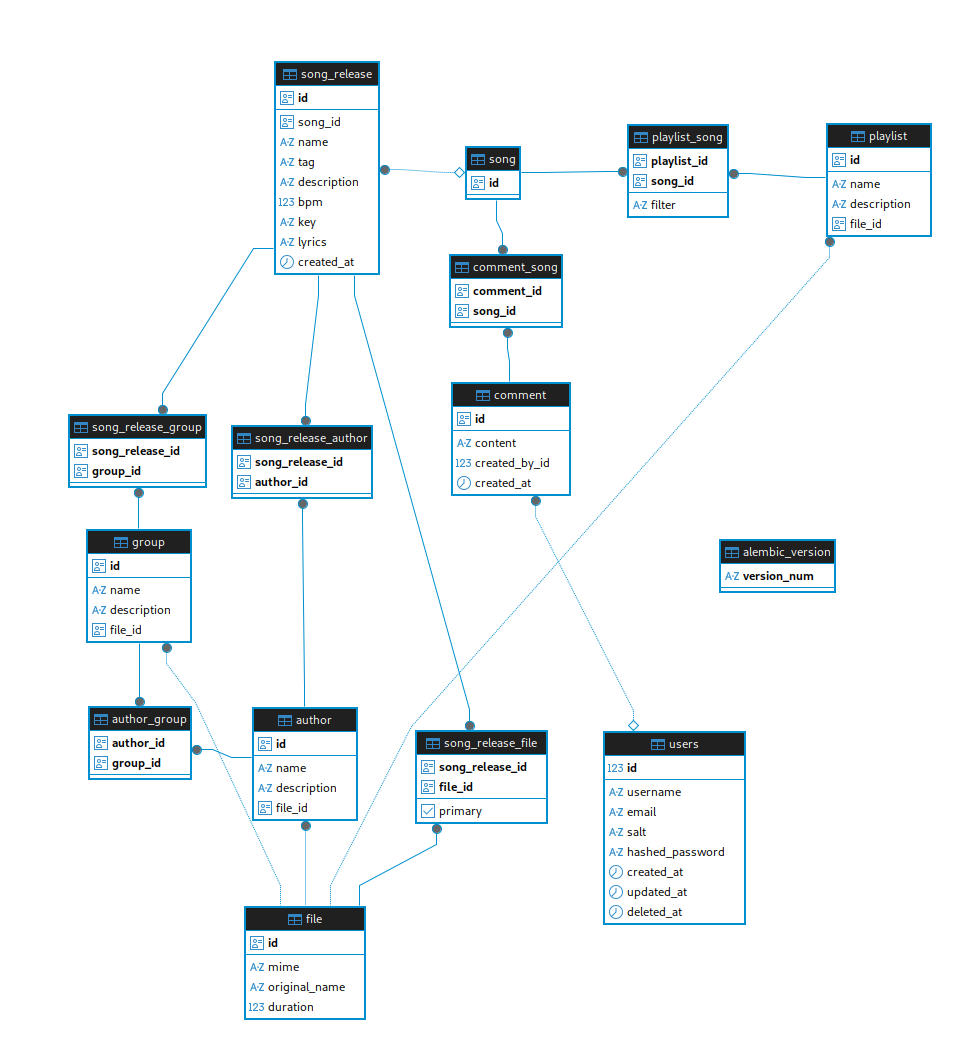
\includegraphics[width=60mm]{figures/pic2_5.png}
    \column{0.5\textwidth}
      \textbf{Аудиоданные:}
      \begin{itemize}
        \item Входной формат: WAV (PCM mono)
        \item Фреймы фиксированной длины: 16\,384 амплитуд ($\approx$0,37с)
        \item Каждый фрейм~--- независимый вектор
        \item После кодирования: сжатый бинарный формат
        \item При передаче: HTTP Chunked Transfer
        \item Распаковка: потоковая, без ожидания всего файла
      \end{itemize}
  \end{columns}
\end{frame}

% ---- СЛАЙД 9: Математические модели ----
\begin{frame}{Математические модели, методы и алгоритмы}
  \begin{columns}[t]
    \column{0.55\textwidth}
      \textbf{Автоэнкодер (нейросетевой кодек):}
      \begin{itemize}
        \item Вход: фрейм $x \in \mathbb{R}^{16384}$ (0,37с, 44,1\,кГц, моно)
        \item Энкодер: $z = f_\theta(x)$,~~$z \in \mathbb{R}^{8192}$~~(сжатие $\times 2$)
        \item Декодер: $\hat{x} = g_\phi(z)$
        \item Функция потерь: MSE + спектральная
        \item Активатор: LeakyReLU
        \item 589\,824\,000 весов; VRAM $\geq$ 16\,ГБ
      \end{itemize}
      \vspace{0.2em}
      \textbf{Гибрид с FLAC:}
      \begin{itemize}
        \item FLAC (кодер Хаффмана) + автоэнкодер
        \item Целевой коэффициент сжатия: $\times 2$
      \end{itemize}
    \column{0.45\textwidth}
      \textbf{Структура сети:}
      \begin{center}
        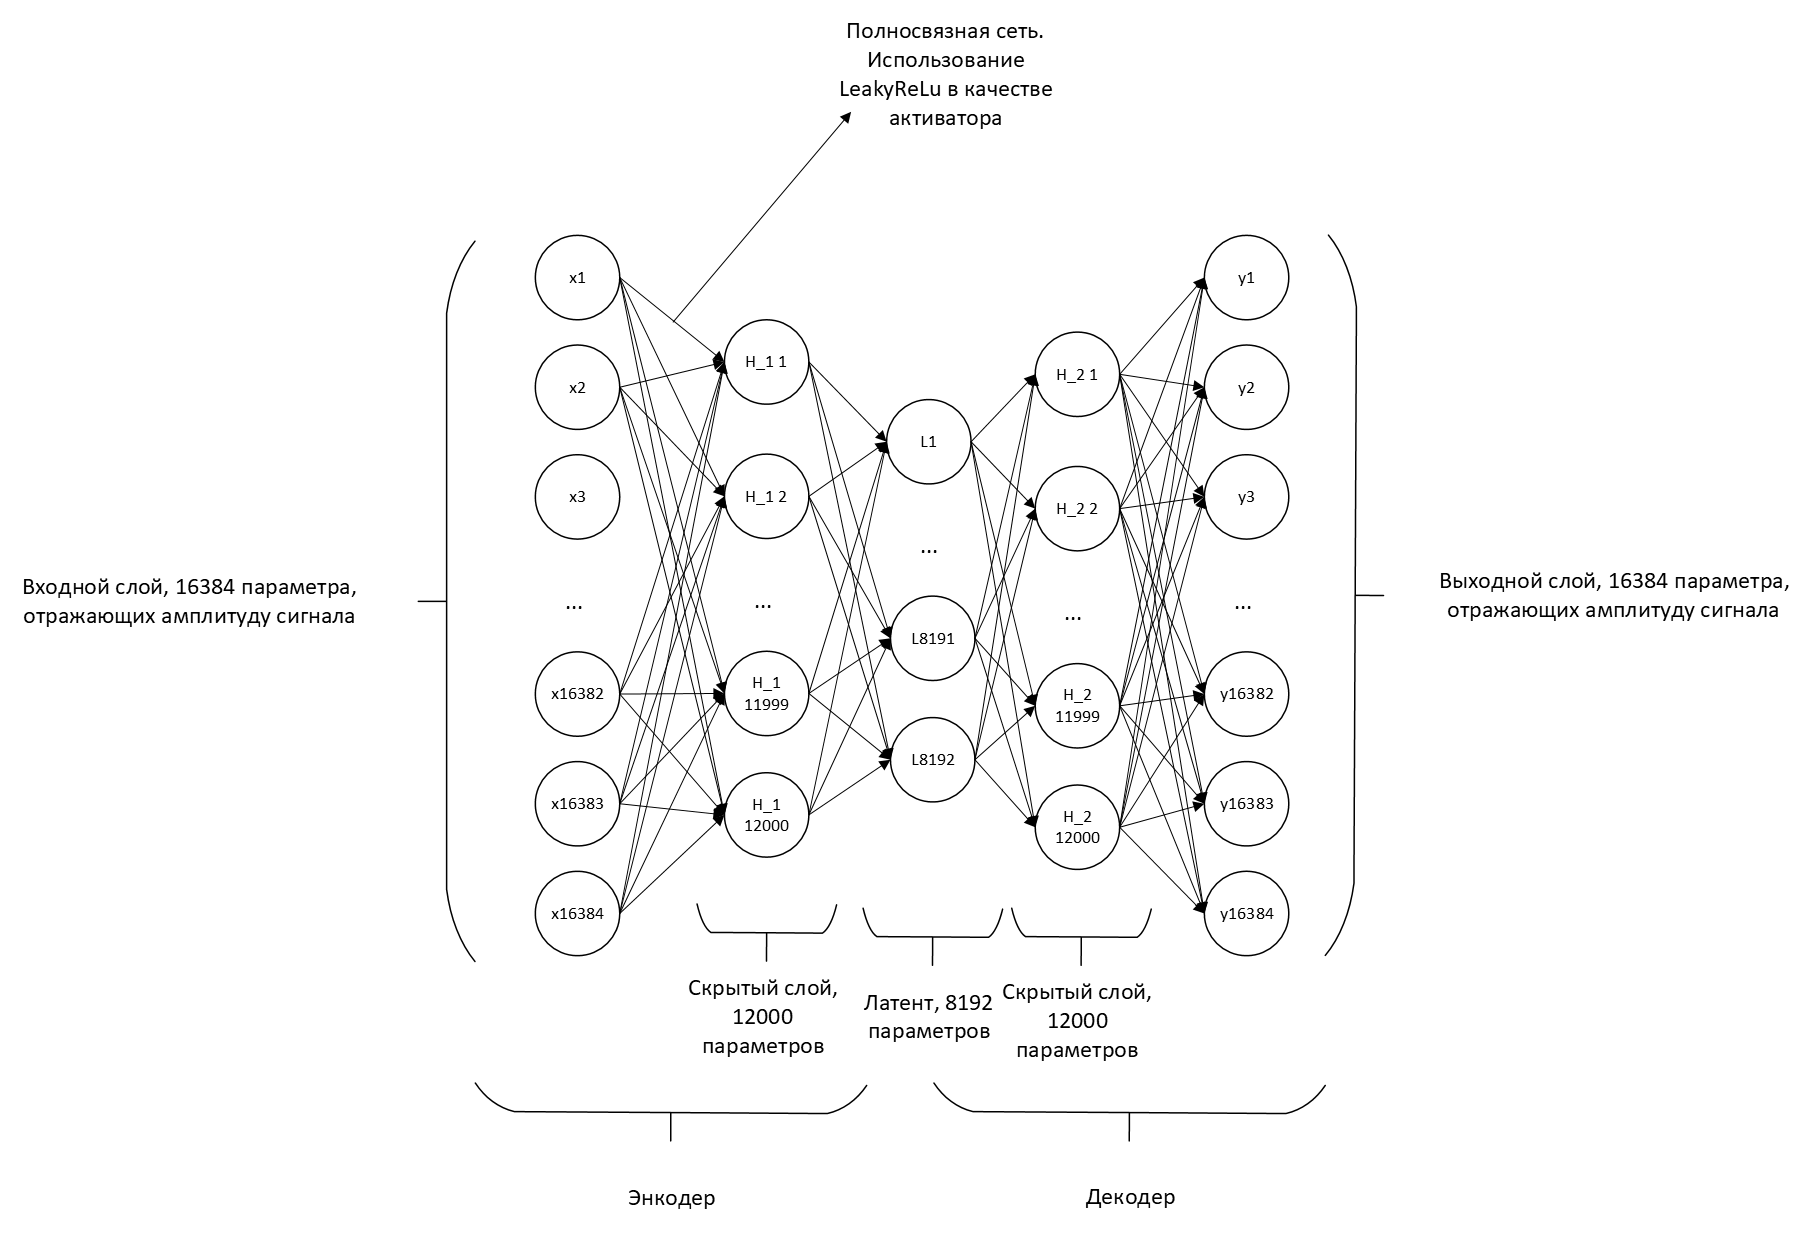
\includegraphics[width=60mm]{figures/pic2_2.png}
      \end{center}
      \vspace{0.3em}
      \textbf{Перцептрон (свёрточные слои):}\\[0.2em]
      Локальные фильтры уменьшают число связей~--- входной слой масштабируется без квадратичного роста параметров.
  \end{columns}
\end{frame}

% ---- СЛАЙД 10: Архитектура ----
\begin{frame}{Декомпозиция и архитектура ПО}
  \begin{columns}[t]
    \column{0.33\textwidth}
      \textbf{Системная архитектура (монолит):}
      \begin{center}
        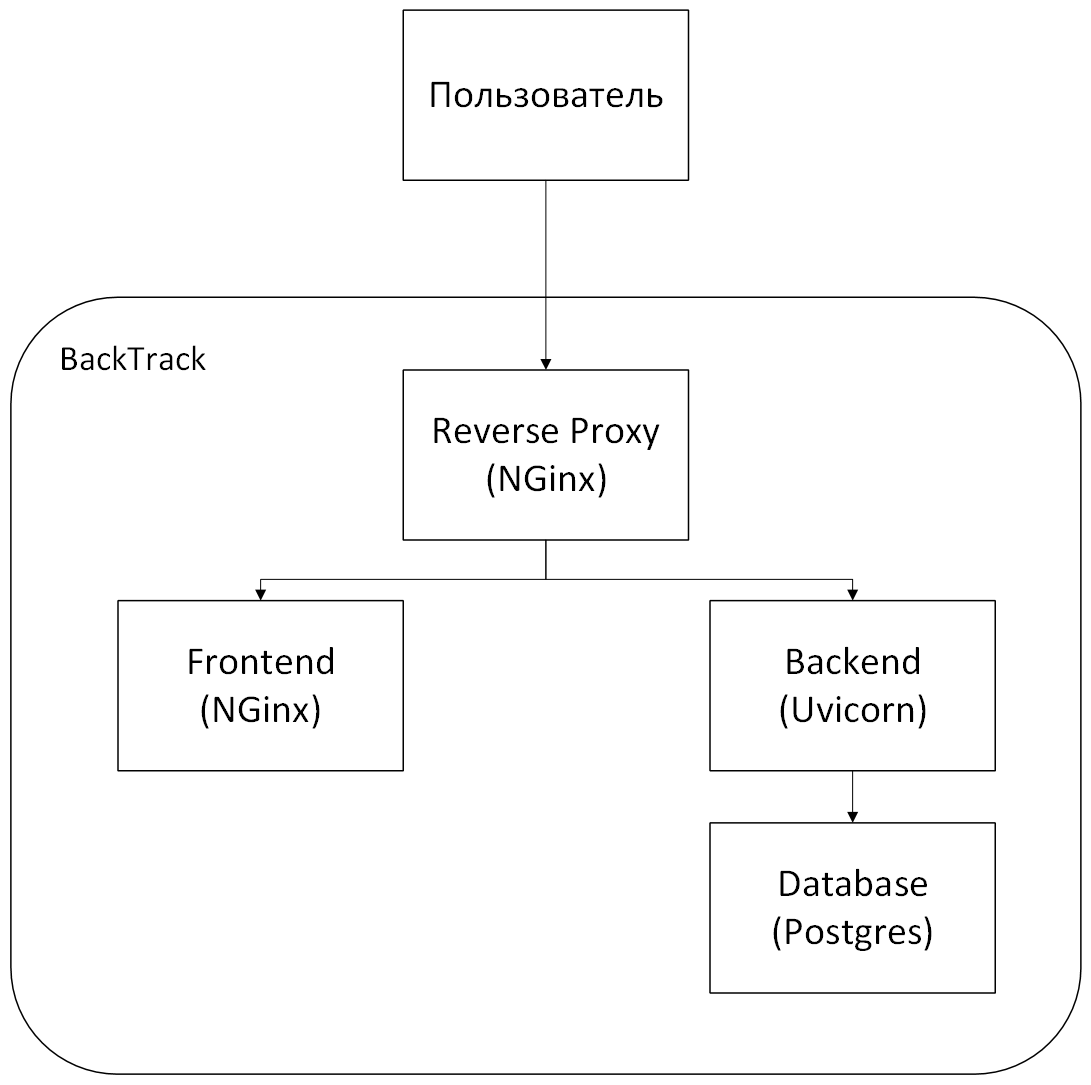
\includegraphics[width=40mm]{figures/networkstruct.png}
      \end{center}
    \column{0.34\textwidth}
      \textbf{Архитектура сервера:}
      \begin{center}
        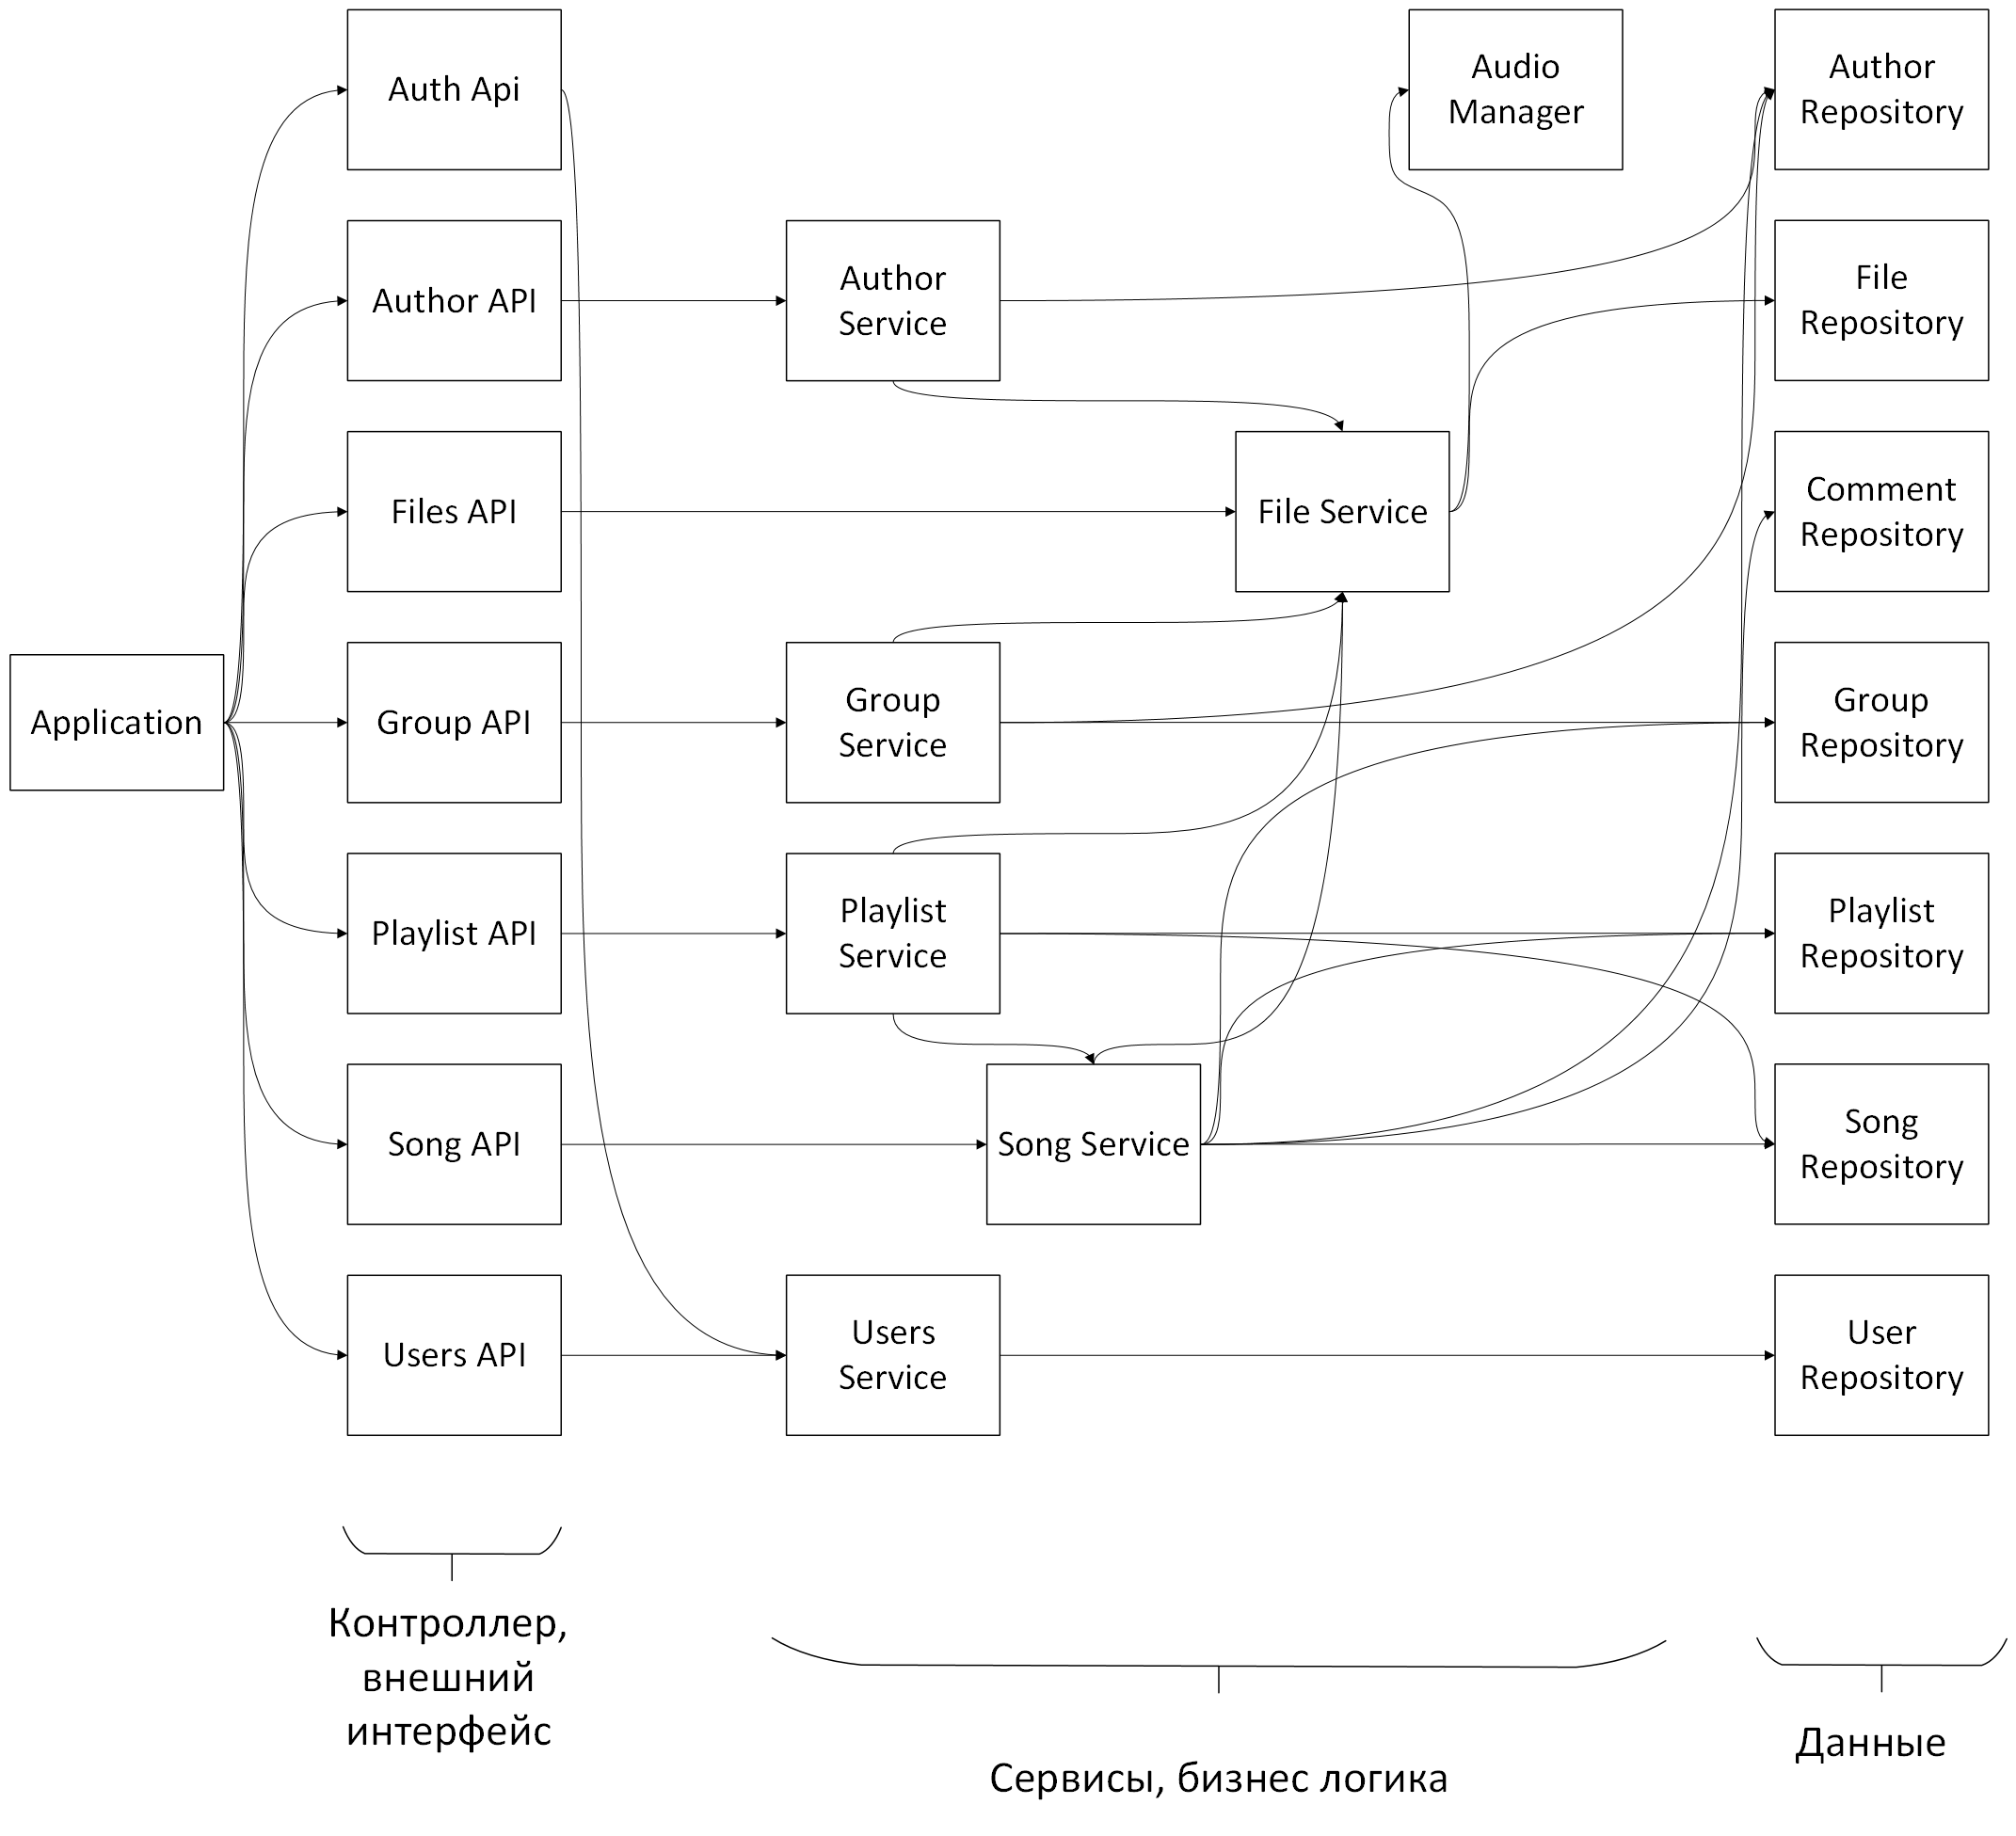
\includegraphics[width=40mm]{figures/pic2_7.png}
      \end{center}
    \column{0.33\textwidth}
      \textbf{Архитектура клиента:}
      \begin{center}
        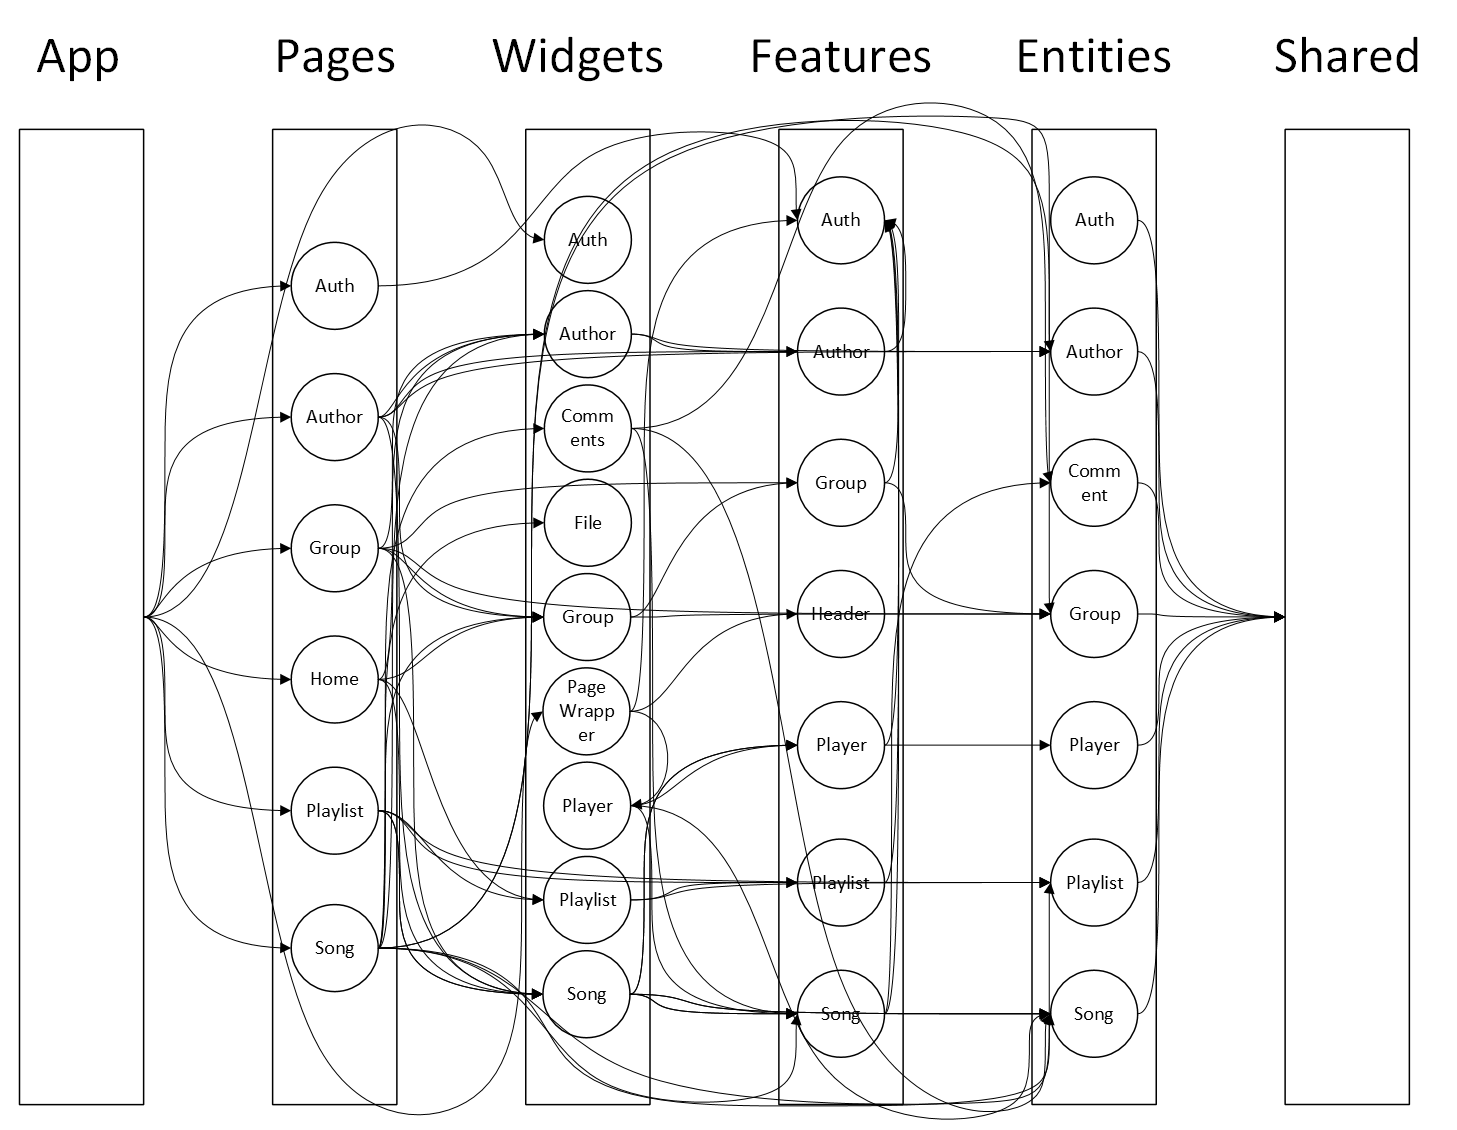
\includegraphics[width=40mm]{figures/pic2_13.png}
      \end{center}
  \end{columns}

  \vspace{0.3em}
\end{frame}

% ---- СЛАЙД 11: Системные требования ----
\begin{frame}{Системные требования}
  \begin{columns}[t]
    \column{0.5\textwidth}
      \textbf{Аппаратура (сервер):}
      \begin{itemize}
        \item CUDA GPU $\geq$16\,ГБ VRAM
        \item ОЗУ $\geq$32\,ГБ
        \item Диск $\geq$1\,ТБ
        \item Канал $\geq$10\,ГБит/с
      \end{itemize}
      \vspace{0.4em}
      \textbf{Клиент:}
      \begin{itemize}
        \item Современный браузер
        \item Канал $\geq$10\,МБит/с
      \end{itemize}
    \column{0.5\textwidth}
      \textbf{ПО (сервер):}
      \begin{itemize}
        \item ОС: Linux (Docker-совместимая)
        \item Docker + Docker Compose
        \item NVIDIA Container Toolkit
        \item CUDA $\geq$ 13.0
        \item Python $\geq$3.10
        \item Node.js (сборка фронтенда)
      \end{itemize}
      \vspace{0.3em}
      Восстановление после отказа: $\leq$1\,часа (ТЗ А.4.2.в)
  \end{columns}
\end{frame}

% ---- СЛАЙД 12: Информационная безопасность ----
\begin{frame}{Методы обеспечения информационной безопасности}
  \begin{columns}[t]
    \column{0.5\textwidth}
      \textbf{Аутентификация и авторизация:}
      \begin{itemize}
        \item JWT в заголовке \texttt{Authorization}
        \item Алгоритм подписи: HS256
        \item Payload: \texttt{id}, \texttt{username}, \texttt{email}
        \item Пароль: bcrypt-хэш + случайная соль
        \item Множественные итерации соли (защита от брутфорса)
      \end{itemize}
    \column{0.5\textwidth}
      \textbf{Защита транспорта и клиента:}
      \begin{itemize}
        \item Pydantic --- валидация всех вх./вых. данных
        \item Авторизация на уровне STOMP WebSocket
        \item Файлы вне БД --- сокращение атакуемой поверхности
        \item Self-hosted: данные не покидают инфраструктуру
      \end{itemize}
  \end{columns}
  \vspace{0.3em}
  {\fontsize{8.5}{10}\selectfont
  JWT хранится в RAM клиента --- CSRF нерелевантен.
  Схемы запросов и ответов разделены во избежание утечки внутренних данных.}
\end{frame}

% ---- СЛАЙД 13: Внешний вид ----
\begin{frame}{Внешний вид программы}
  \begin{columns}[t]
    \column{0.5\textwidth}
      \textbf{Формы:}
      \begin{center}
        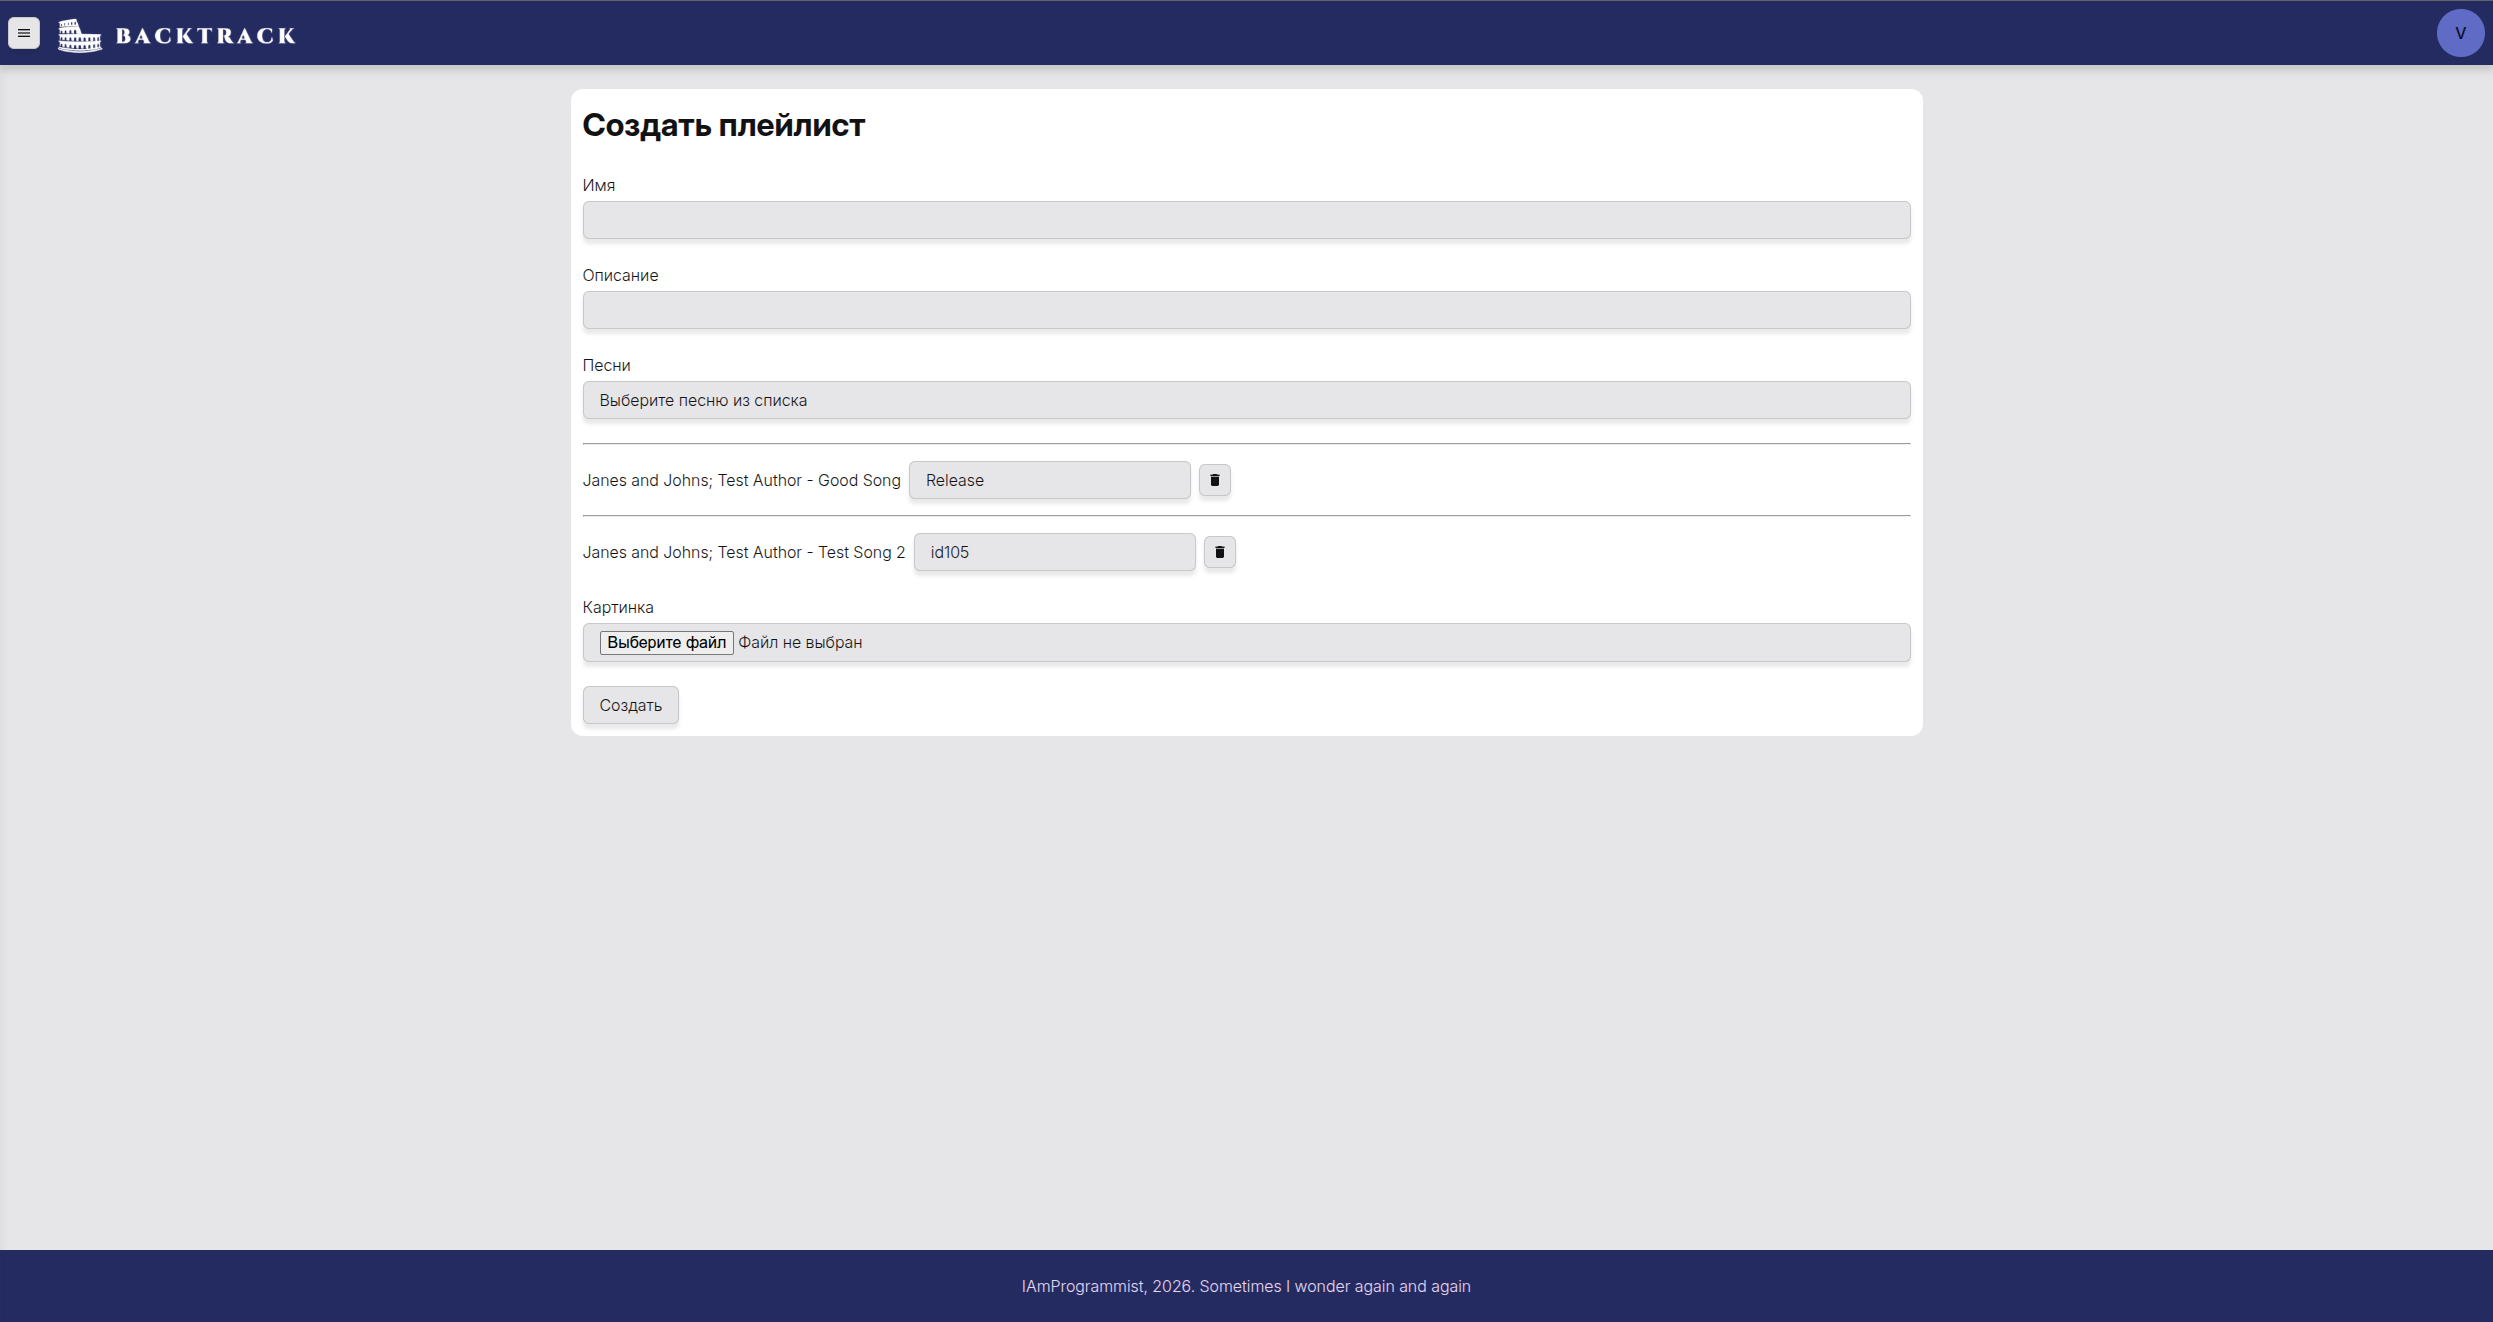
\includegraphics[width=50mm]{figures/pic3_12.png}\\
        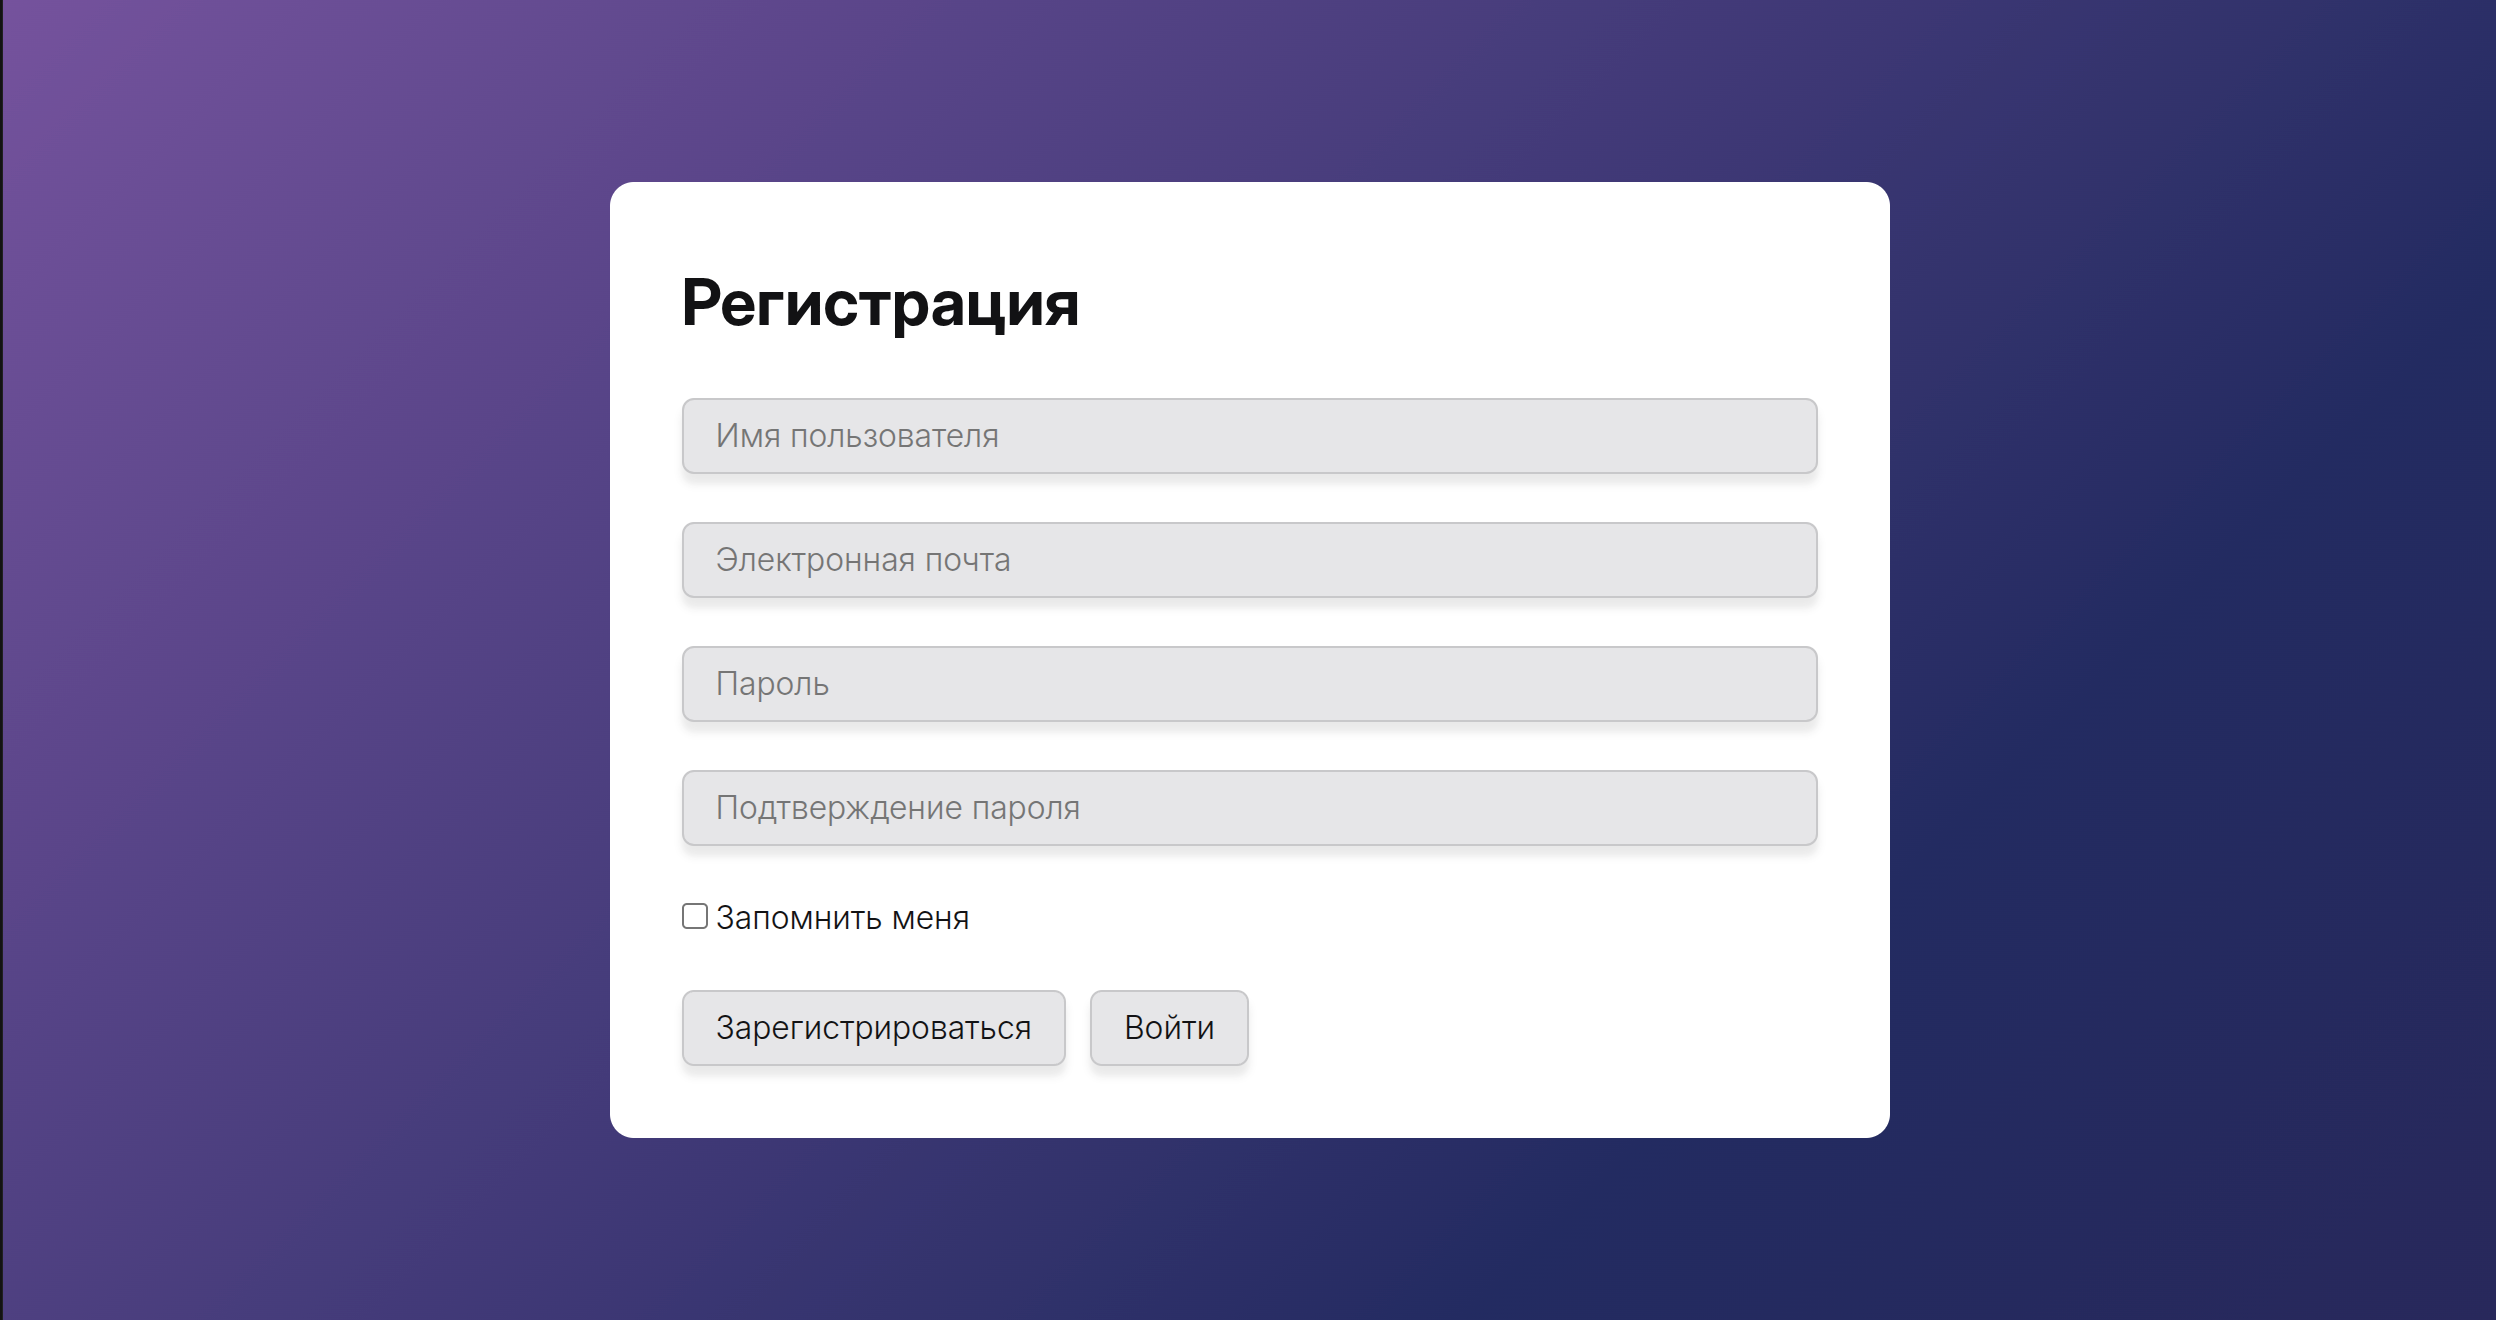
\includegraphics[width=50mm]{figures/pic3_5.png}\\
      \end{center}
    \column{0.5\textwidth}
      \textbf{Основные экраны:}
      \begin{center}
        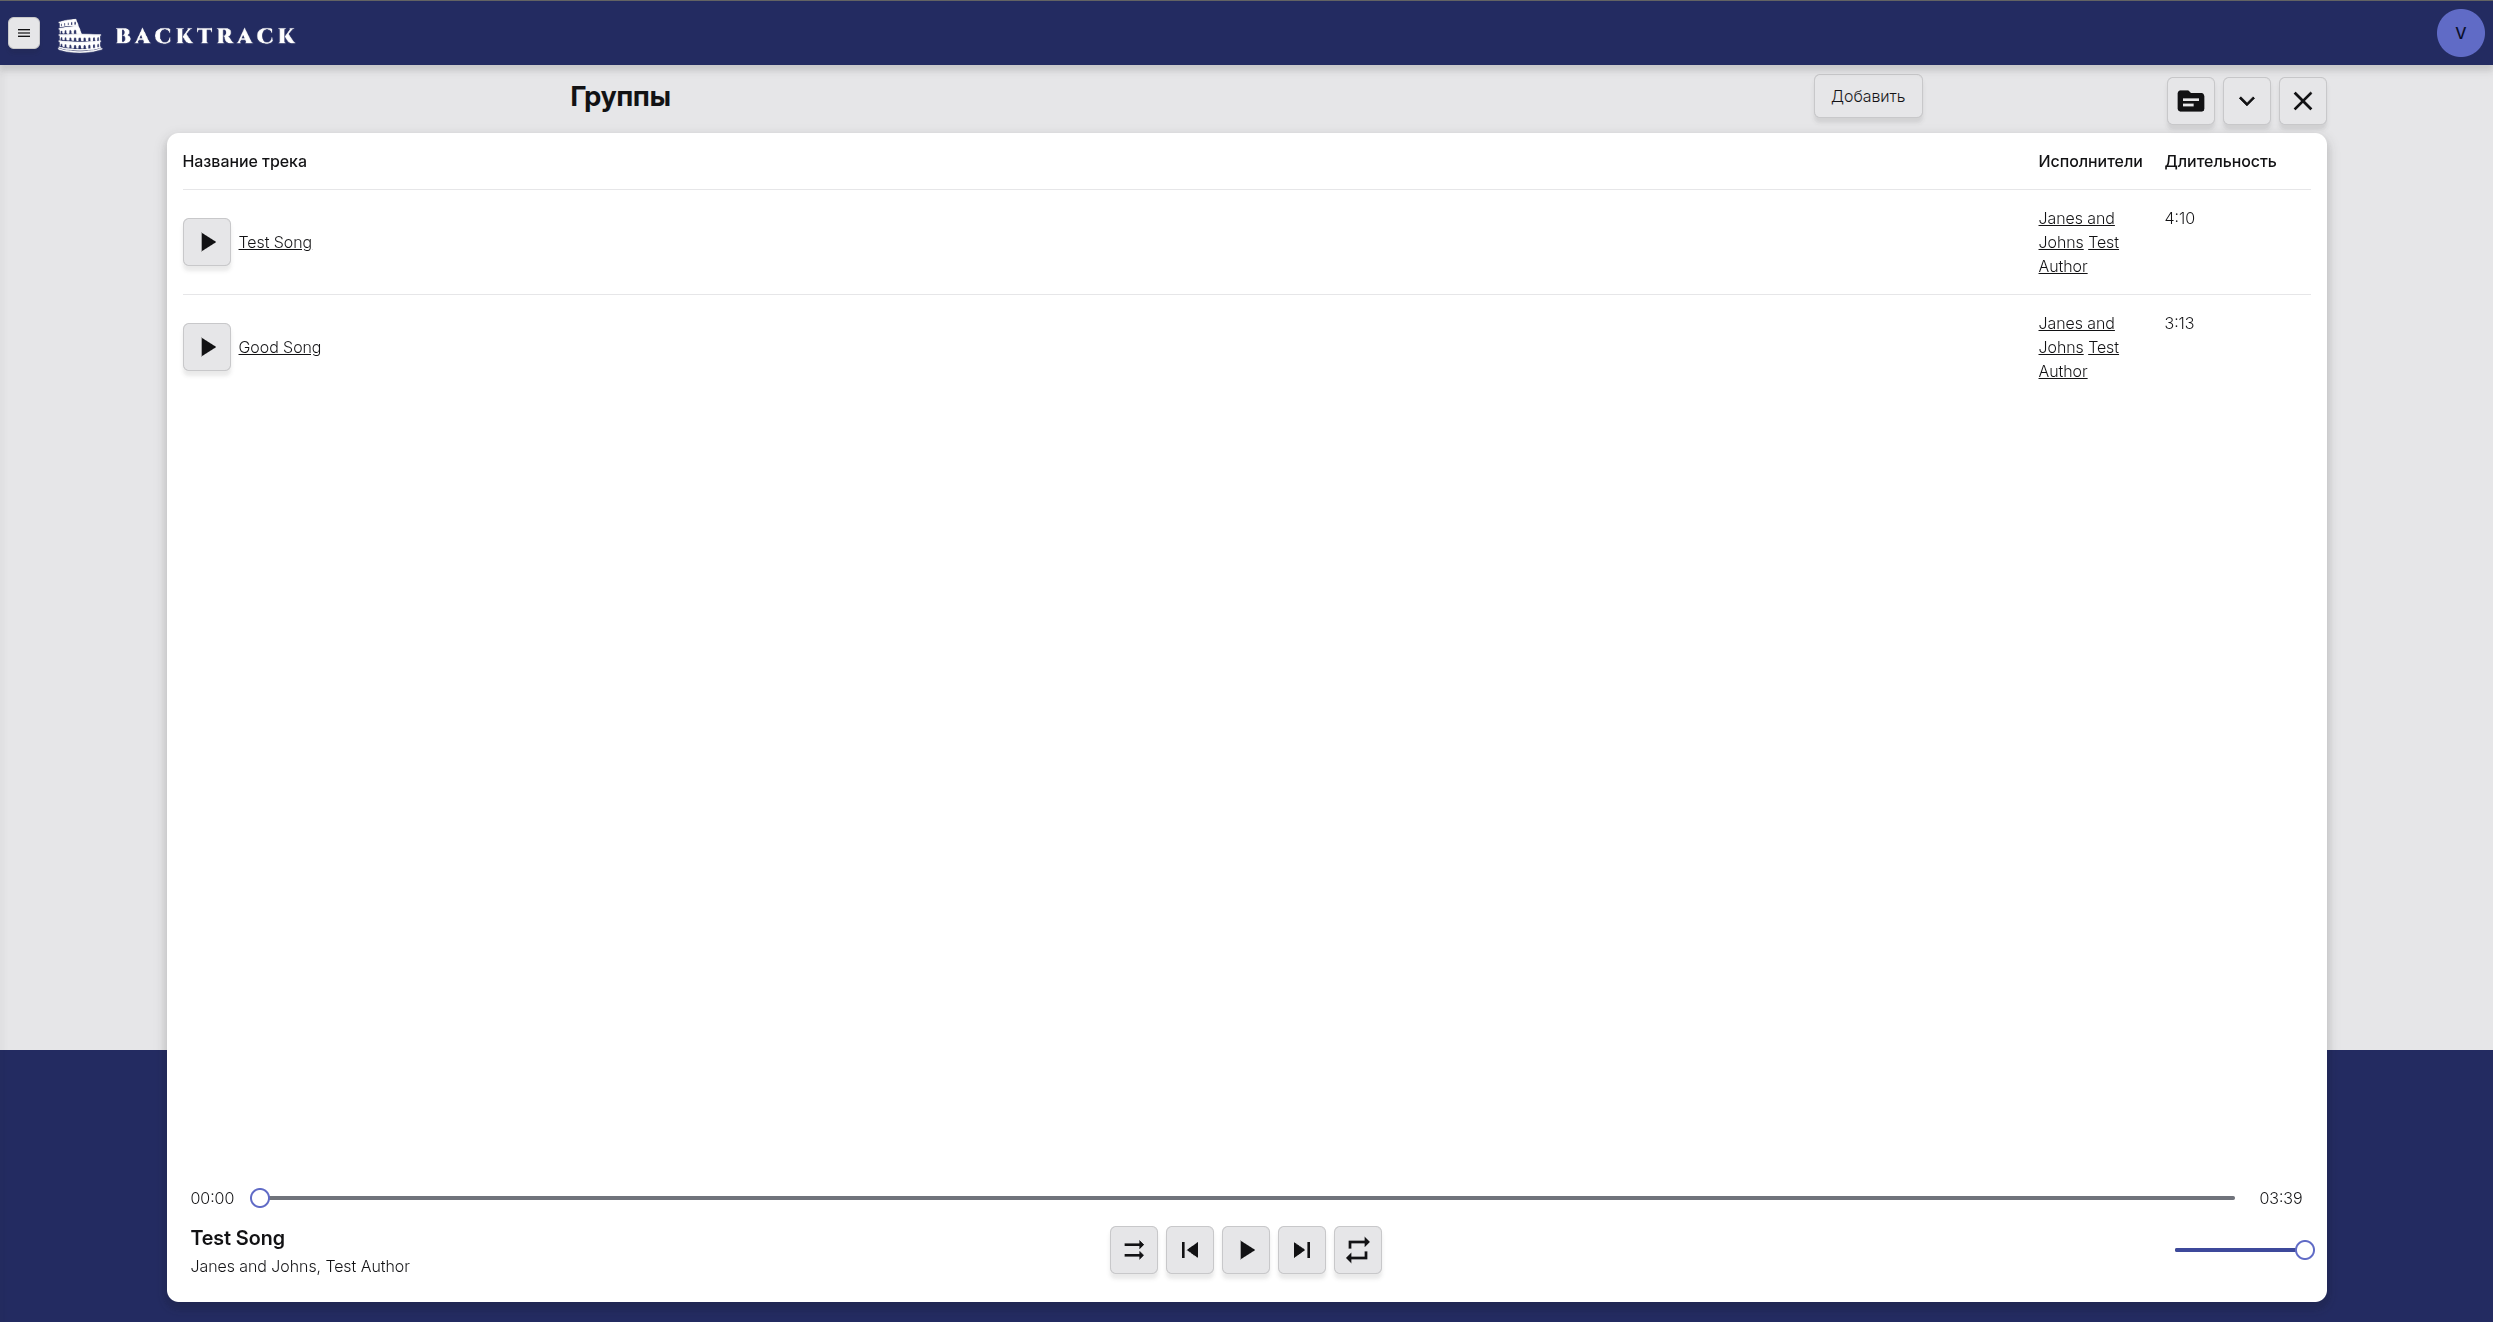
\includegraphics[width=50mm]{figures/pic3_15.png}\\
        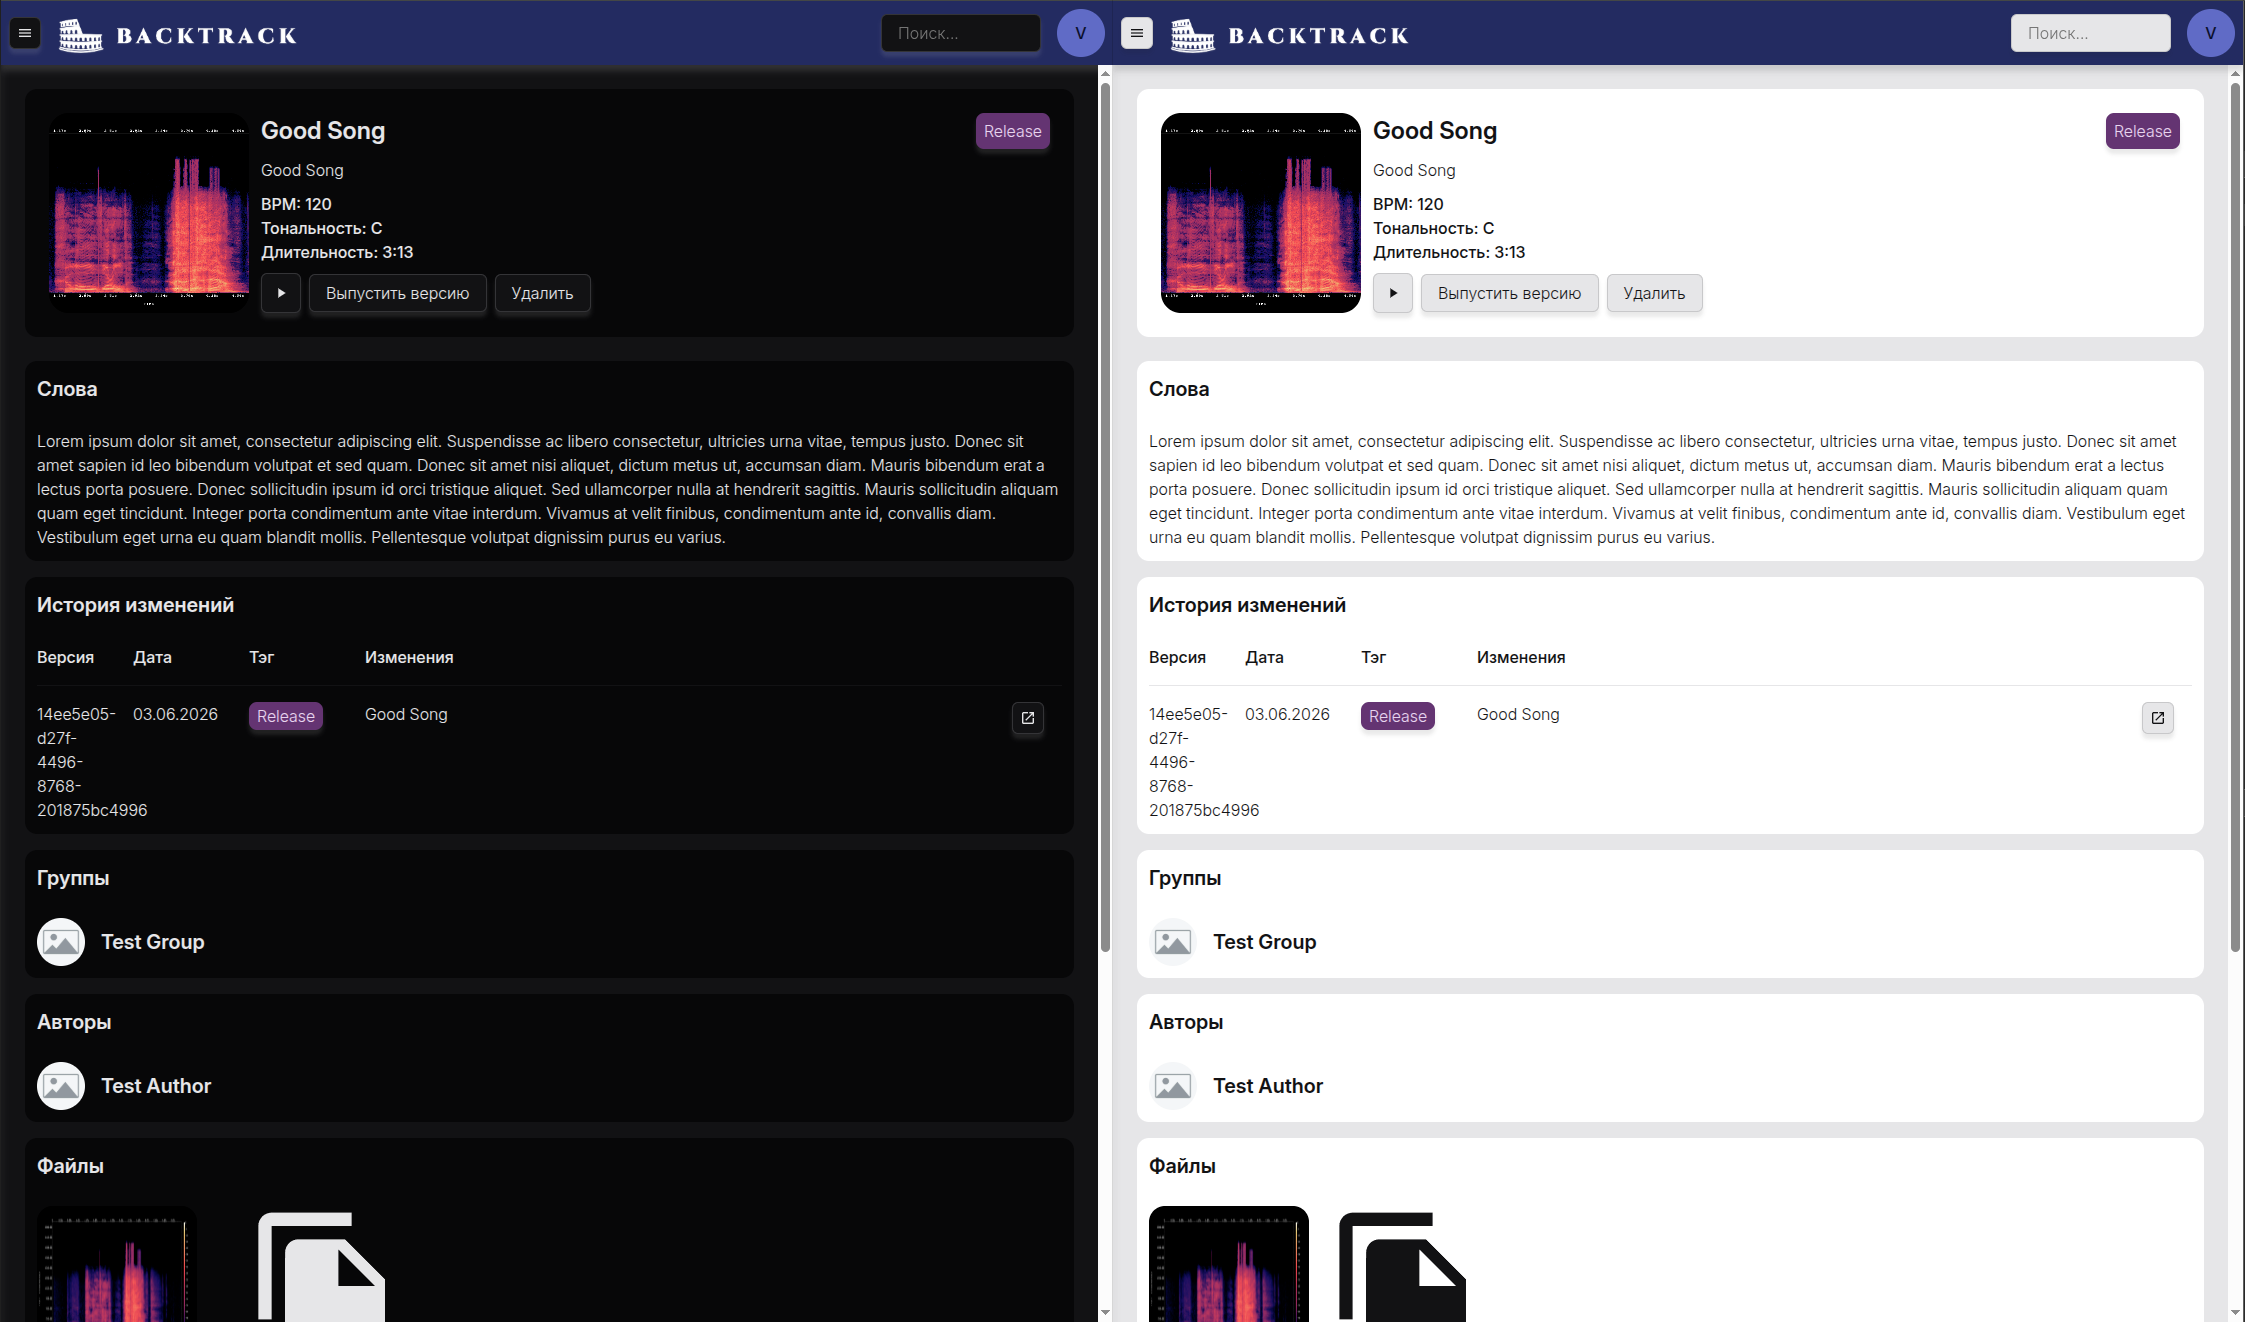
\includegraphics[width=50mm]{figures/pic3_3.png}\\
      \end{center}
  \end{columns}
\end{frame}

% ---- СЛАЙД 14: Результаты экспериментов и тестирования ----
\begin{frame}{Результаты экспериментов и тестирования}
  \begin{columns}[t]
    \column{0.55\textwidth}
      \textbf{Обучение нейронных сетей:}
      \begin{itemize}
        \item Метрики: SNR и \% амплитуд в допуске ($\pm$5/10/20\%)
        \item \textbf{Лучший результат:} SNR~=~17\,дБ (разборчивая речь)
        \item Модель не достигла минимума --- возможно дообучение
        \item Спектральная функция потерь: качество падало с эпохами
        \item Увеличение нейронов в скрытом слое не оправдало затрат
      \end{itemize}
    \column{0.45\textwidth}
      \textbf{Smoke-тестирование:}
      \begin{itemize}
        \item Сценарии по пунктам А.4.1 ТЗ
        \item Пройдены: авторизация, CRUD, версионирование, плейлисты, плеер, загрузка файлов
        \item Healthcheck бэкенда и фронтенда
      \end{itemize}
      \vspace{0.2em}
      \textbf{Потоковая распаковка:}
      \begin{itemize}
        \item HTTP Chunked Transfer подтверждён: воспроизведение начинается до загрузки всего файла
      \end{itemize}
  \end{columns}
\end{frame}

% ---- СЛАЙД 15: Заключение ----
\begin{frame}{Заключение}
  \textbf{В ходе работы разработан и протестирован сервис BackTrack:}
  \begin{itemize}
    \item \textbf{Исследованы} алгоритмы хранения аудио (FLAC, MP3, AAC, Opus); возможности использования гибридной схемы FLAC + автоэнкодер
    \item \textbf{Разработан} сервер на FastAPI + PyTorch + NVIDIA CUDA
    \item \textbf{Разработан} фронтенд на React + RxJS (Feature Sliced Design)
    \item \textbf{Проведено} Smoke-тестирование всех функциональных требований
    \item \textbf{Составлено} руководство пользователя
  \end{itemize}
\end{frame}

\end{document}